 % Eine der drei folgenden Dokumentenklassen muss gewählt werden.
% Für alle Abgaben außer der finalen Endabgabe darf das 'final'
% Schlüsselwort NICHT gesetzt sein.
% Weitere Hinweise sind im Leitfaden zu finden.

%\documentclass[12pt,titlepage,draft]{book}	% Erstellen der Arbeit und Erstabgabe
%\documentclass[12pt,titlepage]{book}		% Korrigierte Erstabgabe
\documentclass[12pt,titlepage,final]{book}	% Finale digitale und gedruckte Abgabe
%\documentclass[oneside]{book}				% Ohne Zwischenseiten

%\usepackage[ngerman]{babel} % Deutsche Version
\usepackage[english]{babel} % Englische Version

\usepackage{iflang}
\usepackage{listings}
\usepackage{acronym}
\usepackage[automake]{glossaries}
\usepackage{em-thesis} 
\usepackage{titlesec}
\titleformat{\chapter}[display]{}{\filleft\scshape\chaptername\enspace\thechapter}{-2pt}{\filright \Huge \bfseries}[\vskip4.5pt\titlerule]
\titleformat{name=\chapter, numberless}[block]{}{}{0pt}{\filright \Huge \bfseries}[\vskip4.5pt\titlerule]

\titlespacing{\chapter}{0pt}{-15pt}{25.5pt}
\titlespacing{name=\chapter, numberless}{0pt}{16pt}{15pt}
% Erweitert Klasse book
% Hier werden automatisch die folgenden Pakete geladen:
% fontenc, inputenc, graphicx, makeidx, fancyhdr, 
% array, colortbl, xcolor, longtable, xspace

% Hier weitere eigene Pakete einfügen
%\usepackage{amsmath} %Erweiterte Satzmöglichkeiten für Mathematik
%\usepackage{mathpazo} %Palatino-Schrift

% hyperref sollte als letztes Paket geladen werden; dieses ermöglicht Links in PDF
% Hinweis: Die Verwendung von hyperref fuehrt noch zu identifier-Warnungen wg.
%          unterschiedlicher Seitennummerierung.
%\usepackage[plainpages=false, pdfpagelabels]{hyperref}

%\usepackage[dvipdfm]{graphicx}
%\usepackage{bmpsize}


\makeglossaries
\newglossaryentry{Aaa}{name={ERM},description={Entity Relationship Model}}
\newglossaryentry{Bbb}{name={UML},description={Unified modelling language}}
\newglossaryentry{Ccc}{name={BPMN},description={Business Process Modelling Notation}}
\newglossaryentry{Ddd}{name={EPC},description={Event - driven process chain}}
\newglossaryentry{Eee}{name={BPMS},description={Business Process Management System}}
\newglossaryentry{Fff}{name={BPMI},description={Business Process Management Initiative}}
\newglossaryentry{Ggg}{name={OMG},description={Object Managment Group}}
\newglossaryentry{Hhh}{name={BPMN 2.0},description={Business Process Modelling Notation 2.0}}
\newglossaryentry{Iii}{name={CMMN},description={Case Management Model and Notation}}
\newglossaryentry{Jjj}{name={DMN},description={Decision Management Notation}}
\newglossaryentry{Kkk}{name={IT},description={Information Technology}}
\newglossaryentry{Lll}{name={REST},description={Representational State Transfer pattern}}
\newglossaryentry{Mmm}{name={SOAP},description={Simple Object Access Protocol}}
\newglossaryentry{Nnn}{name={XML},description={Extended Markup Language}}
\newglossaryentry{Ooo}{name={KPI},description={Key Performance Indicator}}
\newglossaryentry{Ppp}{name={TAL},description={Teilnehmeranschlussleitung; english: local loop}}
\newglossaryentry{IVR}{name={IVR},description={Interactive Voice Response}}
\newglossaryentry{Qqq}{name={MSA},description={Microservice Architecture}}
\newglossaryentry{SAFe}{name={SAFe},description={Scaled Agile Framework for}}
\newglossaryentry{DEVOP}{name={DevOps},description={Development and IT Operation}}
\newglossaryentry{MS}{name={MS},description={Microservice}}
\newglossaryentry{WSBPEL}{name={WS-BPEL},description={Webservice-Business Process Execution Language}}
\newglossaryentry{jpdl}{name={jPDL},description={jBPM Process Definiton Language}}

%\newglossaryentry{Incl}{name={incl.},description={includes [something]}}
%\newglossaryentry{eg}{name={e.g.},description={for example}}
%14



%%Informationen fuer die Titelseite
\thesisauthor{
	David Adam and
	Patrick Schuster
}
\matrikel{
	58126, 57562}
\thesistype{}
\thesistitle{Analysis and evaluation of modelling languages and \\ workflow engines}
%\thesisleiter{Dipl. Ing. Lucia Mejia Dorantes}
%\thesissupervisors{B. Sc. Jonas Hansert} % Form bei einem Betreuer
\thesissupervisors[B. Sc. Jonas Hansert]{Dipl. Ing. Lucia Mejia Dorantes} % Form bei zwei Betreuern
%Startdatum ist optional, bei Nichtgebrauch einfach die Zeile löschen oder auskommentieren
\thesisenddate{20th\ January 2020}



% Beispiele für Trennhilfen, falls Fremdworte oder Spezialausdrücke nicht richtig getrennt werden
% Wichtig! 
% Im german-paket sind zusätzlich folgende Trennhinweise enthalten:
% "- = zusätzliche Trennstelle
% "| = Vermeidung von Ligaturen und mögliche Trennung (bsp: Schaf"|fell)
% "~ = Bindestrich an dem keine Trennung erlaubt ist (bsp: bergauf und "~ab)
% "= = Bindestrich bei dem Worte vor und dahinter getrennt werden dürfen
% "" = Trennstelle ohne Erzeugung eines Trennstrichs (bsp: und/""oder)

% Trennhinweise für Wörter hier beschreiben
\hyphenation{
% Pro-to-koll-in-stan-zen
% Ma-na-ge-ment  Netz-werk-ele-men-ten
% Netz-werk Netz-werk-re-ser-vie-rung
% Netz-werk-adap-ter Fein-ju-stier-ung
% Da-ten-strom-spe-zi-fi-ka-tion Pa-ket-rumpf
% Kon-troll-in-stanz
}

%\makeindex
\begin{document}
% 

%\begin{onehalfspacing}
\ifoptionfinal{}{%
\IfLanguageName{ngerman}{
	%\thispagestyle{empty}
%% Beginn Deckblatt
%\fbox{%
%\parbox{.9\textwidth}{%
%{\Huge Fassung vom \today} \\[1em]
%{\Large \textbf{Achtung:} Dieses Deckblatt ist \textbf{nicht} Bestandteil der gebundenen Fassung dieser Arbeit! Es dient nur zur Versionskontrolle, falls z.\,B.\ vorgezogene Abgaben an den Betreuer stattfinden. Für die finale digitale Abgabe kann das Einbinden an der entsprechenden Stelle in der Hauptdatei unterbunden werden.
%Dazu muss der Status des Dokuments auf 'final' gesetzt werden.}
%}
%}
%\vfill
%\clearpage
%\blankpage




}{
	\include{em_includes/coversheet_en}
}
\blankpage % Leerseite auf Titelrückseite
}

% Titelseite einbinden
\IfLanguageName{ngerman}{
	%% Titelseite
%% Vorlage $Id: titelseite.tex,v 1.2 2001/01/24 20:13:25 bless Exp bless $
\titlehead{
	\includegraphics*[width=4cm]{em_includes/hskaLogo} \hfill
	\includegraphics*[width=4cm]{em_includes/IUMS} 	
} % end titlehead
%\titlehead{\includegraphics*[width=4cm]{em_includes/hskaLogo}}

\begin{titlepage}
%\let\footnotesize\small \let\footnoterule\relax
\begin{center}

\hbox{}
\vfill
{\usebox{\thesistitlesaveone}\par}
\vskip 1cm
\usebox{\thesistypesave}\\
Literature review in\\
\medskip
Transportsystem management B.Sc. at\\
Institute of Ubiquiturious Mobilitysystems\\
Faculty Informationmanagement and Media\\
University of Applied Science\\[2ex]
written by\\[2mm]
\textbf{\usebox{\thesisauthorsaveone}}\\
\vspace*{\baselineskip}
Student number: \\
\begin{tabular}{l}
	\usebox{\thesismatrikelsave} \\
\end{tabular}
\vskip 1.5cm
Supervisor: \\[2mm]
\begin{tabular}{l}
%\usebox{\thesisleiter}\\
\usebox{\thesissupervisortwosave} \\
\end{tabular} \\ [2mm]
Leading Supervisor: \\[2mm]
\begin{tabular}{l}
	%\usebox{\thesisleiter}\\
	\usebox{\thesissupervisoronesave} \\
\end{tabular}


\vskip 1.5em
\begin{tabular}{ll}
\ifthenelse{\boolean{startdatumtext}}{Tag der Anmeldung: &}{}
\usebox{\thesisstartdatesave} \\
Submission date: & \usebox{\thesisenddatesave} \\
\end{tabular}

\vspace*{3em}
% add versioning information
%\ifoptionfinal{}{%
%	\ifoptiondraft{%
%		\Large\drafttext{Draft}%
%	}{%
%		\Large\drafttext{Preprint}%
%	}
%}
\end{center}
\vfill
\end{titlepage}
%% Titelseite Ende


}{
	%% Titelseite
%% Vorlage $Id: titelseite.tex,v 1.2 2001/01/24 20:13:25 bless Exp bless $
\titlehead{
	\includegraphics*[width=4cm]{em_includes/hskaLogo} \hfill
	\includegraphics*[width=4cm]{em_includes/IUMS} 	
} % end titlehead
%\titlehead{\includegraphics*[width=4cm]{em_includes/hskaLogo}}

\begin{titlepage}
%\let\footnotesize\small \let\footnoterule\relax
\begin{center}

\hbox{}
\vfill
{\usebox{\thesistitlesaveone}\par}
\vskip 1cm
\usebox{\thesistypesave}\\
Literature review in\\
\medskip
Transportsystem management B.Sc. at\\
Institute of Ubiquiturious Mobilitysystems\\
Faculty Informationmanagement and Media\\
University of Applied Science\\[2ex]
written by\\[2mm]
\textbf{\usebox{\thesisauthorsaveone}}\\
\vspace*{\baselineskip}
Student number: \\
\begin{tabular}{l}
	\usebox{\thesismatrikelsave} \\
\end{tabular}
\vskip 1.5cm
Supervisor: \\[2mm]
\begin{tabular}{l}
%\usebox{\thesisleiter}\\
\usebox{\thesissupervisortwosave} \\
\end{tabular} \\ [2mm]
Leading Supervisor: \\[2mm]
\begin{tabular}{l}
	%\usebox{\thesisleiter}\\
	\usebox{\thesissupervisoronesave} \\
\end{tabular}


\vskip 1.5em
\begin{tabular}{ll}
\ifthenelse{\boolean{startdatumtext}}{Tag der Anmeldung: &}{}
\usebox{\thesisstartdatesave} \\
Submission date: & \usebox{\thesisenddatesave} \\
\end{tabular}

\vspace*{3em}
% add versioning information
%\ifoptionfinal{}{%
%	\ifoptiondraft{%
%		\Large\drafttext{Draft}%
%	}{%
%		\Large\drafttext{Preprint}%
%	}
%}
\end{center}
\vfill
\end{titlepage}
%% Titelseite Ende


}
\blankpage % Leerseite auf Titelrückseite

% Erklaerung einbinden
\IfLanguageName{ngerman}{

%\thispagestyle{empty}
%\vspace*{36\baselineskip}
%\hbox to \textwidth{\hrulefill}
%\par
%Ich versichere hiermit wahrheitsgem\"a{\ss}, die Arbeit selbst\"andig angefertigt, alle benutzten Hilfsmittel vollst\"andig und genau angegeben und alles kenntlich gemacht zu haben, was aus Arbeiten anderer unver\"andert oder mit Ab\"anderung entnommen wurde.

%Ich stimme der Publikation dieser Arbeit auf der Webseite der Abteilung f\"ur Informationsdienste und elektronische M\"arkte des Instituts f\"ur Informationswirtschaft und Marketing am Karlsruher Institut f\"ur Technologie (KIT) zu.

%Karlsruhe, den \usebox{\thesisenddatesave}

%\clearpage





}{
% Auch im Englischen bleibt Declaration auf Deutsch!

%\thispagestyle{empty}
%\vspace*{36\baselineskip}
%\hbox to \textwidth{\hrulefill}
%\par
%Ich versichere hiermit wahrheitsgem\"a{\ss}, die Arbeit selbst\"andig angefertigt, alle benutzten Hilfsmittel vollst\"andig und genau angegeben und alles kenntlich gemacht zu haben, was aus Arbeiten anderer unver\"andert oder mit Ab\"anderung entnommen wurde.

%Ich stimme der Publikation dieser Arbeit auf der Webseite der Abteilung f\"ur Informationsdienste und elektronische M\"arkte des Instituts f\"ur Informationswirtschaft und Marketing am Karlsruher Institut f\"ur Technologie (KIT) zu.

%Karlsruhe, den \usebox{\thesisenddatesave}

%\clearpage





}
\blankpage % Leerseite auf Erklaerungsrückseite

%% Verzeichnisse
\pagenumbering{Roman}
\setcounter{page}{4}
\let\cleardoublepage\clearpage %Skips blank pages and adds one blank page behind cover
\addcontentsline{toc}{chapter}{List of Abbrevations}

\tableofcontents
%\blankpage
\printglossary[title={List of Abbreviations}] %Generate List of Abbreviations
%\blankpage
\addcontentsline{toc}{chapter}{List of Figures}
\listoffigures   % Falls gewuenscht, Kommentarzeichen am Anfang entfernen.
%\blankpage
\addcontentsline{toc}{chapter}{List of Tables}
\listoftables    % Falls gewuenscht, Kommentarzeichen am Anfang entfernen.
%\blankpage



%% Hauptteil
\pagenumbering{arabic}


%%%%%%%%%%%%%%%%%%%%%%%%%%%%%%%%%%%%%%%%%%%%%%%%%%%%%%%%%%%%%%%%%%%%%%%%%%%%%%%%%%%%%%%%
% Hier beginnt die eigenstaendige Ausarbeitung
%%%%%%%%%%%%%%%%%%%%%%%%%%%%%%%%%%%%%%%%%%%%%%%%%%%%%%%%%%%%%%%%%%%%%%%%%%%%%%%%%%%%%%%%

% Tipp: Anstatt direkt hier LaTeX-Code einzutippen, kann der Inhalt in anderen Dateien
%       abgelegt werden und per \input bzw. \include eingebunden werden.
%       Der Unterschied zwischen \input und \include ist der fehlende Seitenvorschub bei 
%       \input
\begin{onehalfspacing}
\setcounter{page}{0}
%--------------------------------------------------------------------------
%READ ME

%How to bibliography BUT first export on citavi
%Hinblickend auf Mobilitätsentwicklung führt der ÖV an, waren es im Jahr 1994 noch 12,3 \% stieg die Verkehrsleistung pro Person um nahezu das Doppelte auf 21,8 \% in 2014 \cite{MOP}. 

%How to footnote
%\footnote{\url{http://www.hoc.kit.edu/labore.php, Seite 47 und 49}}\\

% How to insert pictures
%\begin{figure}[!hb]
%	\centering
%	\includegraphics[scale=0.7]{userStory}
%	\caption{Beispielhafte User Story}
%\end{figure}

%HOw to inset numeric list
%\begin{enumerate} %[!hb]
%	\item \textbf{Project Scoping} 
%	\\ some text
%	\item \textbf{Design/ Implementation}
%	\\some txt
%	\\some txt
%	\item \textbf{Solution Rollout}
%	\\some txt
%\end{enumerate}

% How to insert bullet points
%\begin{itemize} %[!hb]
%\item Prognostizierter Besetzungsgrad einzelner Stadtlinien 
%\item Detaillierte Informationen zu Haltestellen 
%\item Fahrgastbewegung an Haltestellen und Bezirke 
%\item Echtzeit Besetzungsgrad und Besetzungsverlauf 
%\end{itemize}

% \textit{accident} -> Italicized
% \textbf{greatest} -> Bold
% \underline{science} -> Underlined

%\makeglossaries -> Abkürzungsverzeichnis anlegen
%\newglossaryentry{Aaa}{name={ERM},description={Entity Relationship Model}} -> Abkürzung anlegen
%  \gls{Aaa} -> Abkürzung aus thesis.tex in content.tex einfügen 

\chapter{Introduction}

\section{Motivation}
In an increasingly information-driven and connected world, we are moving away from simple contexts and clear plausibilities. At the same time, the degree of complexity in a multitude of systems and technical realizations is increasing, making it the task of engineers to document these complexities in an abstract representation. Meaning, Models can transform the complexity of any system into a simple mostly graphic representation. Models are very important for todays software development, in fact they enhance the whole process of documenting and developing on large scope of software products because models help developers to understand the complexity behind the software.\\ 
In \cite{BranSelic.2003}, Bran Selic describes advantages of models in the software development process. More precise, he says that models are implementation and technology indepentend, closer to the problem domain and they enable the generation of artifacts like program code from models.



\section{Background and principles}
Recapping the independent attribute of models and todays complex environment, models need to indicate the difference between irrelevant and relevant objects. Therefore engineers mainly distinguish in system and system context while the irrelevant environment keeps objects which are not considered in the system architecture (Figure 1.1). \\
Borders between system and system context need to be defined for a better grasp of a system architecture. Requirements outside of the context border shall not be considered in the building process which allows a development process to be more stable, time and cost efficient.  \\
A system context analysis examines relevant stakeholder, processes, systems, documents and events that have greater impact on the behaviour of the system. 
The system context represents linked aspects to the system, like subsytems, stakeholder and events by being directly linked through interfaces at the system border to the systems itself. \cite{Pohl.2015} 

\newpage
According to \cite{Bernroider.2006} models follow fundamental principles, the main principles are likely to summarize in: 

\begin{itemize}
	\item \textbf{Abstraction} 
	\\ 
	Abstraction is a natural way of describing and classifying use cases. But objects in a model can be defined in a percise way too which leads often to an interplay between abstraction and concretion of a system.
	\item \textbf{Partitioning} 
	\\
	As already mentioned by the definiton of system context, Partitioning considers subsystems. The core aspect of partitioning is modelling \textit{abstracted} interfaces and objects before to define precisely the individual structure.
	\item \textbf{Projection} 
	\\
	Misguided projection can lead to incompleted models which turns into insufficient and unsustainable system development. Projection takes different points of view into consideration, especially those of the different type of users and stakeholders. For example: The developer has a different view of the system than someone from management whose biggest satisfaction lies in user experience and covering cost-efficient requirements.
	\item \textbf{Modelling languages} 
	\\
	Modelling languages cover a wide range of deployment which is guided by standardisation e.g. ISO, rules and symbols. This lecture review will concentrate on main modelling languages whose can be applied into the phases of software development and give a fundamental understanding of model-based software engineering.
\end{itemize}


\begin{figure}[!hb]
	\centering
	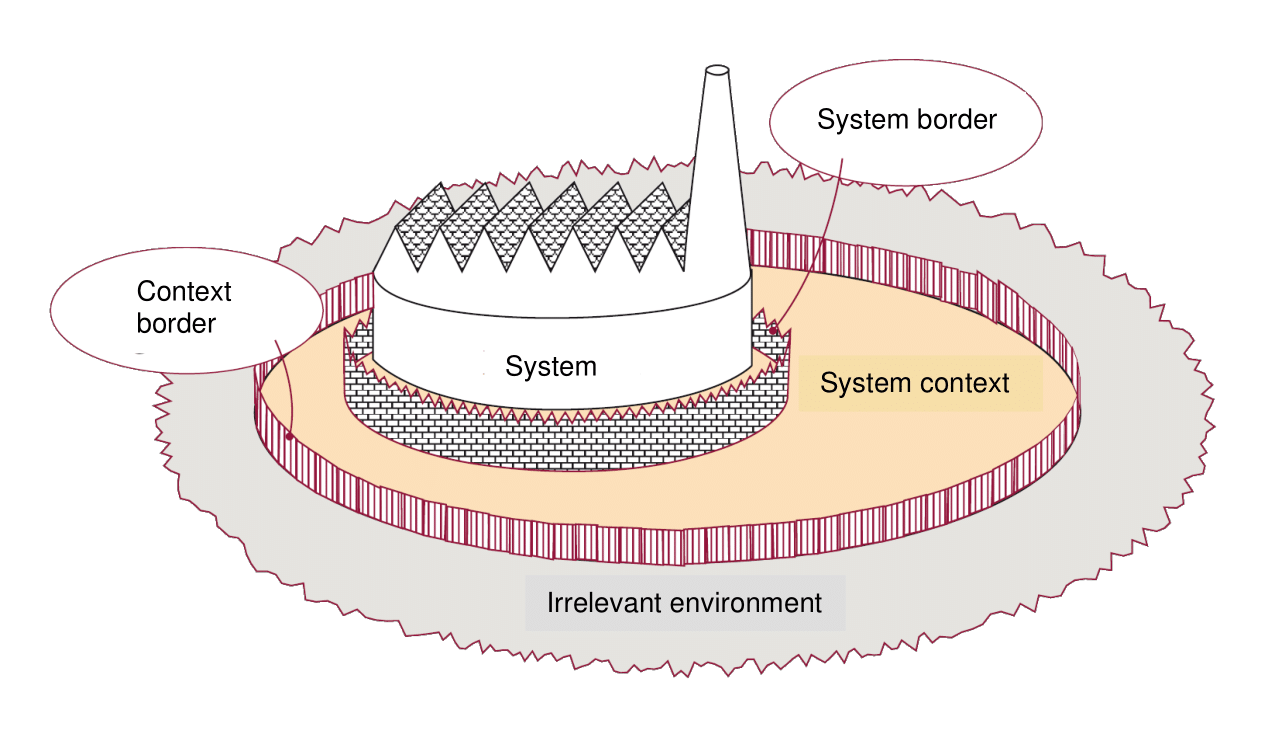
\includegraphics[scale=0.6]{SystemAndContext}
	\caption{Abstracted difference between system and system context. \cite{AmelieLang.2019}}
\end{figure}


\newpage
\chapter{Modeling languages}

A model is an abstract image of an existing or yet to be created reality \cite{Stachowiak.1973}.
\\
Besides natural language, system-requirements are often specified and documented by modelling languages. In general, experts map their functional system-requirements into three perspectives; Behaviour-, structure- and functional perspective (Figure 2.1).\\


\begin{figure}[!hb]
	\centering
	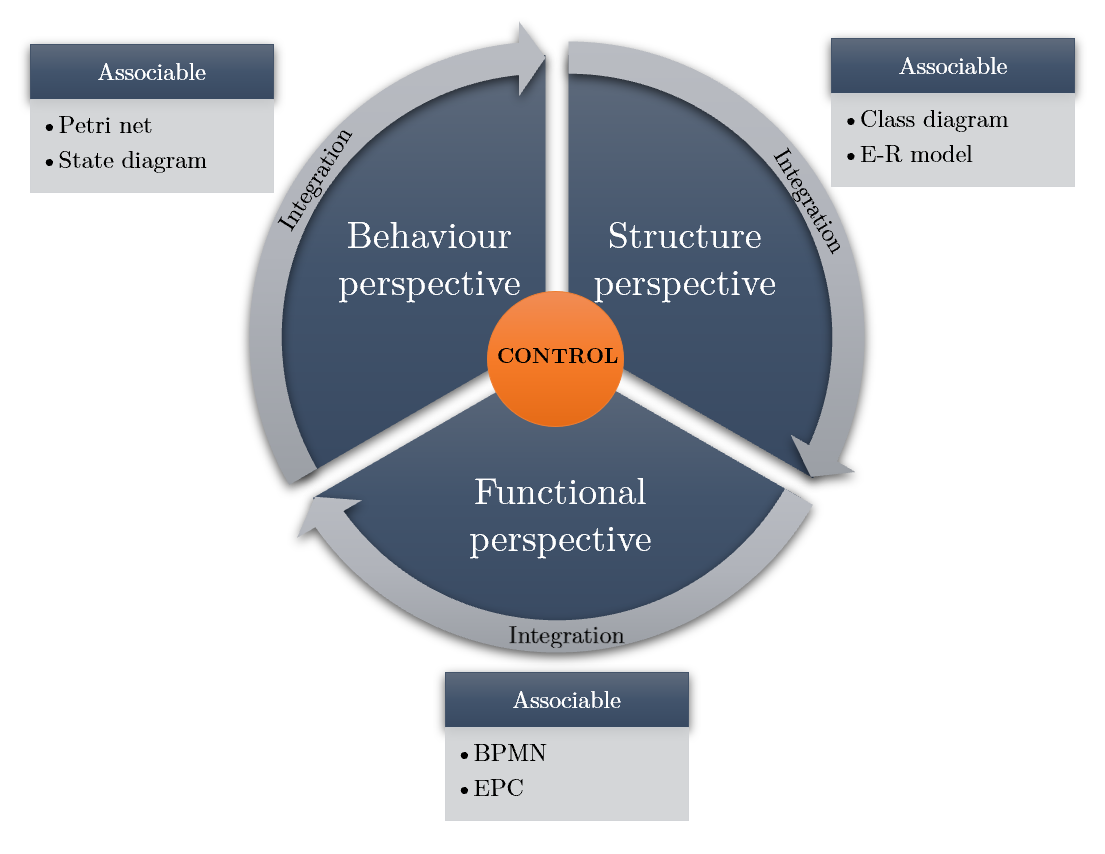
\includegraphics[scale=0.7]{PerspektivenModel}
	\caption{Model-based documentation divided into three perspectives.}
\end{figure}


Besides that, the illustration provides for each perspective an exemplarily set of modelling languages. For example, static data is modelled in class diagrams, object flow activities are found in the behaviour perpective as state diagrams and typically represent a functional perspective. \cite{Pohl.2015} \\
Model-based requirements help to apply artefacts in a cross-functional team based on hard-level of formalisations and specified semantic for integration patterns. \\[3em]


\newpage
\section{Structural perspective}
The structure perspective is a relevant modelling approach for the communication of mostly static-data and structure between systems and subsystems.

\subsection{Entity-relationship model}
The data modelling is an essential point in software development. A entity-relationship model (\gls{Aaa}) abstracts the structure and establishes semantics between systems and databases. Therefore, this language focuses on the abstraction of databases modelled in relational, object-oriented and networked data models.
ERM is characterized by modelling static views of use cases and data, which does not mean that requirements towards process cycles or transformations can be ignored. Instead, the engineer is required to use modeling languages according to their areas of application and capabilities \cite{Bernroider.2006}. \\
Following the principle of \textit{abstraction}, ERM proposes two main elements (Table 2.1) to realize abtracted and highly acceptable models. The low complexity of the realization helps to present solutions infront of all types of stakeholder that are involved in the product life cycle.
\begin{table}[!hb]
	\centering
	\label{tbl:TableLatexShortened}
	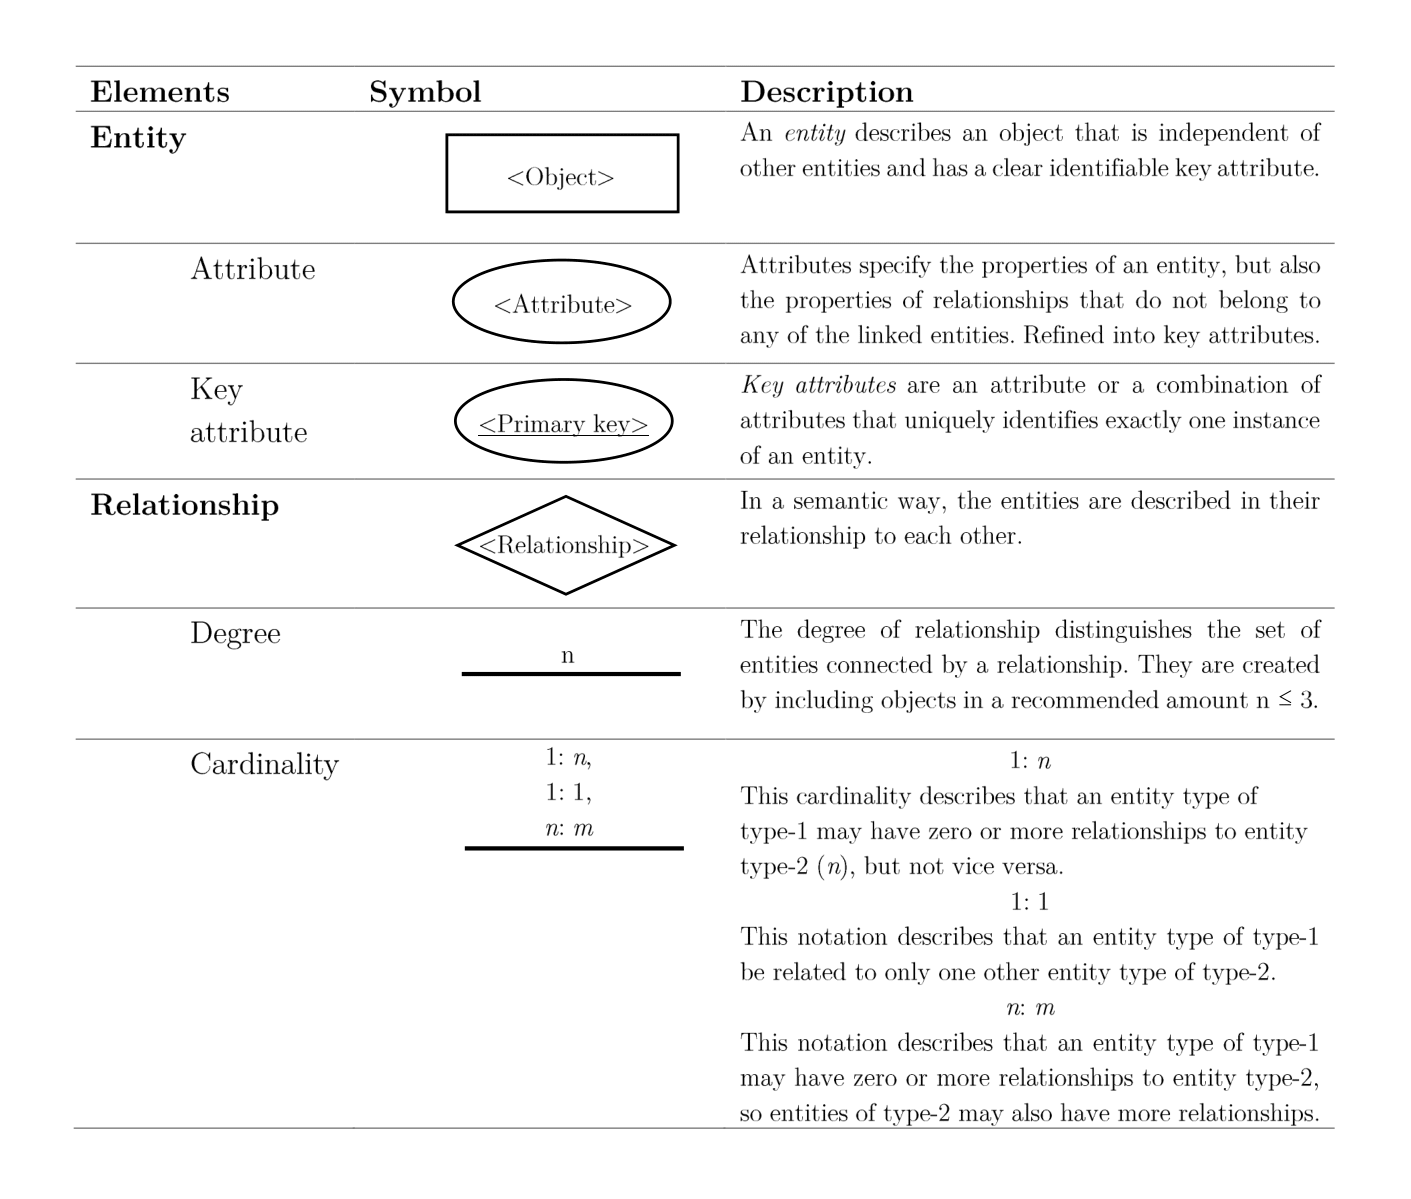
\includegraphics[scale=0.3]{TableLatexShortened}
	\caption{Tabular arrangement of Entity-relationship model elements.}
\end{table}


ERM provides abstracted information about static data between a set of entities. Figure 2.2 applies common ERM symbols to model a use case of booking a rental bike. The example is divided by three entity types, two relationships and their individual attributes whereas the attributes of "ShareBike" is substantiated in a database table. Moreover, the table "ShareBikeGrid" describes and points out that relationship types and entity types are differentiated to their very own instances (so-called tuples). \\


\begin{figure}[!hb]
	\centering
	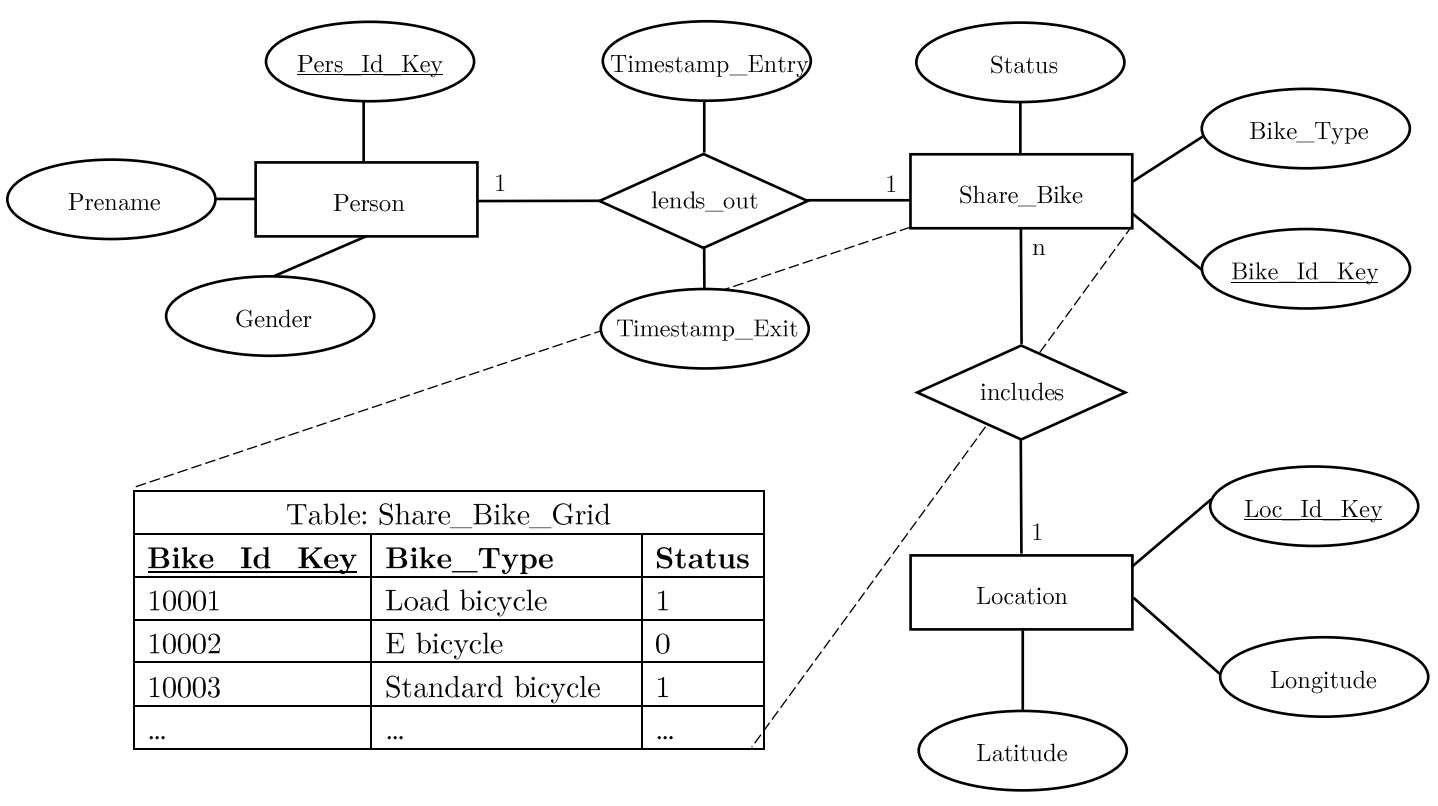
\includegraphics[scale=0.6]{ERMexample}
	\caption{Example of an ERM with rental bike scenario.}
\end{figure}


\subsection{Class diagram (UML)}
Founded in 1997 by the Object Management Group, Unified Modeling Language (\gls{Bbb}) has established itself as one of the most widely used modeling languages. \cite{EdSeidewitz.2003} Basically, modeling with \gls{Bbb} can be divided into two types. Static modeling is performed by the class diagram, while dynamic modeling is performed by sequence diagrams or state diagrams. In this chapter the most important parts of the class diagram are shown, which describes the structural perspective of the system. In particular, the UML class diagram is frequently used to describe the structure of a software system and thus forms the first basis for object-oriented modeling. The UML Classdiagramm combines the ideas of the Entity-Relationship modeling and the graphic representation of modules \cite{Benker.2016}. Consequently the class diagram achieves a greater cardinality in the description of objects, for example classes \cite{Pohl.2015}.
\\
Over the years, the ERM has become standard for the description of database models.\cite{ShamkantB.Navathe.1992} However, according to the results from (\cite{AndreaDeLuciaCarmineGravinoRoccoOlivetoGenoveffaTortora.2008}, \cite{AndyS.Evans.1998}), UML significantly simplifies the understanding of data models but has deficits when it comes to deduce properties about it. In addition, the use of UML class diagrams is less effective when it comes to specific questions about the relationships between two objects. Nevertheless UML is benefical for software engineering.
Vargas et al \cite{RutTorresVargasAriadiNugrohoMichelChaudronJoostVisser.2012} found that “at the system level, the change
proneness of code modeled using class diagrams is lower
than that of code that is not modeled at all.” 
\newpage
The following table (Table 2.2) shows the essential elements of a UML class diagram.
\begin{table}[!hb]
	\centering
	\label{tbl:TableLatexShortened}
	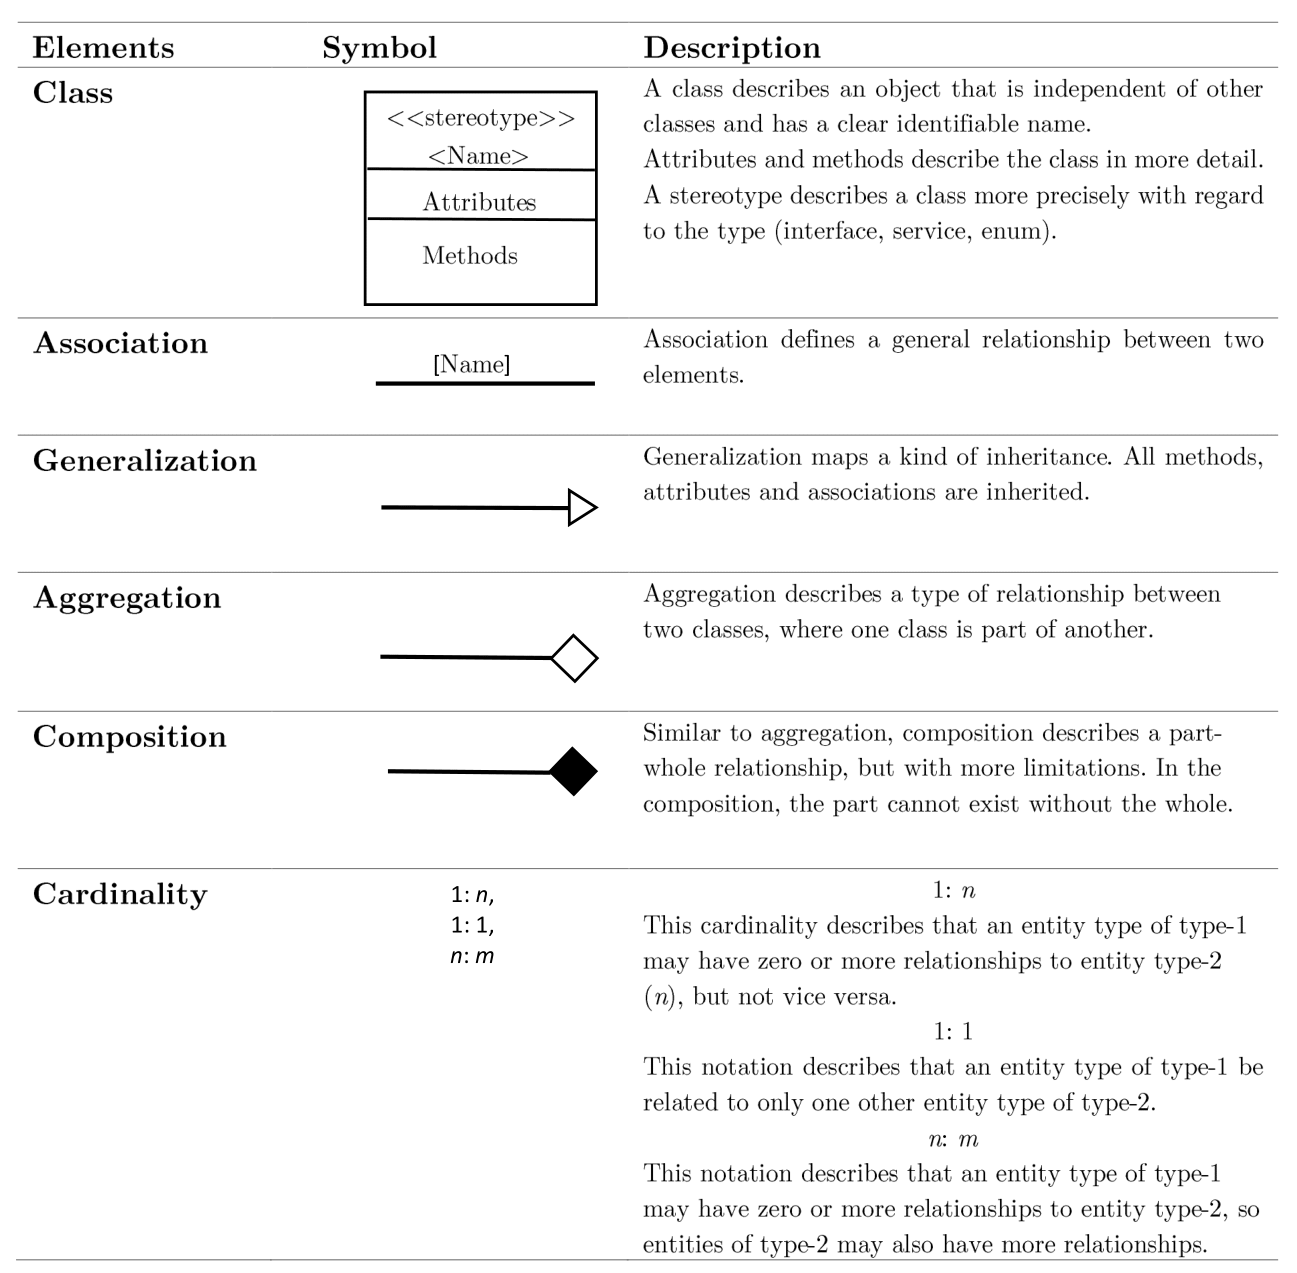
\includegraphics[scale=0.3]{ExampleUML-1}
	\caption{Tabular arrangement of UML model elements.}
\end{table}

By transforming the example from the ERM, we get a more compact and understandable representation of the system in Figure 2.3. Following the model based approach we can directly derive domain objects from the model, due to the more exact description of the classes. 
\begin{figure}[!hb]
	\centering
	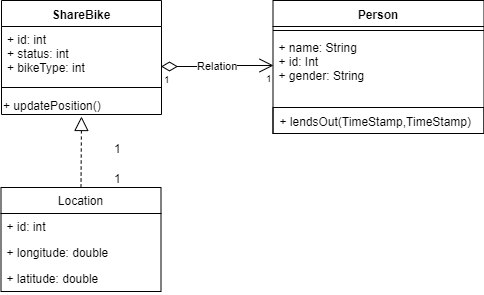
\includegraphics[scale=0.6]{UMLExample}
	\caption{Example of an UML Classdiagram with rental bike scenario.}
\end{figure}

\newpage
\section{Functional perspective}
In the functional perspective, the functionalities (which are available to the user) of a technical system are modelled in its system environment. Functional perspective considers the information in the system context, that is manipulated by a systematic event from the system.



\subsection{Event-driven process chain}
The Event-driven process chain is a modelling language used for describing business processes. \gls{Ddd} aims to describe processes at the business logic level and not necessarily at the formal specification level. \cite{G.KellerM.NuttgensA.W.Scheer.Januar1992} Therefore, the strength of EPC modeling lies in its easy-to-understand notation, which makes it possible to map business information systems and simultaneously integrate properties such as functions, data, organizational structures and information resources.\cite{Benker.2016} \\
One of the central deficits is that the semantics of an EPC are not clearly defined and it is also not possible to check the model for consistency and completeness. \cite{Krogstie.2012} In contrast to structure modeling, process models always describe a dynamic view within an information model.\cite{G.KellerM.NuttgensA.W.Scheer.Januar1992} \\
In a EPC, the process-related context is represented by functions. Functions are triggered by a starting-event. While events trigger the start of a function events can also be determined as a result of a function. There are a few important semantic restrictions to EPC, which are as follows.\cite{MuhammadWaseemAnwar.March132018}

\begin{itemize}
	\item  
	Events cannot make decisions like OR/XOR decisions.
	Events can only be linked with AND operator.
	\item 
	Functions can be associated with all three logical operators
	(AND, OR, XOR) for decision making.
	\item 
	Additional process objects can only be connected with
	the functions of EPC.
\end{itemize}


\newpage
The following table shows the essential elements of an EPC model

\begin{table}[!hb]
	\centering
	\label{tbl:TableLatexShortened}
	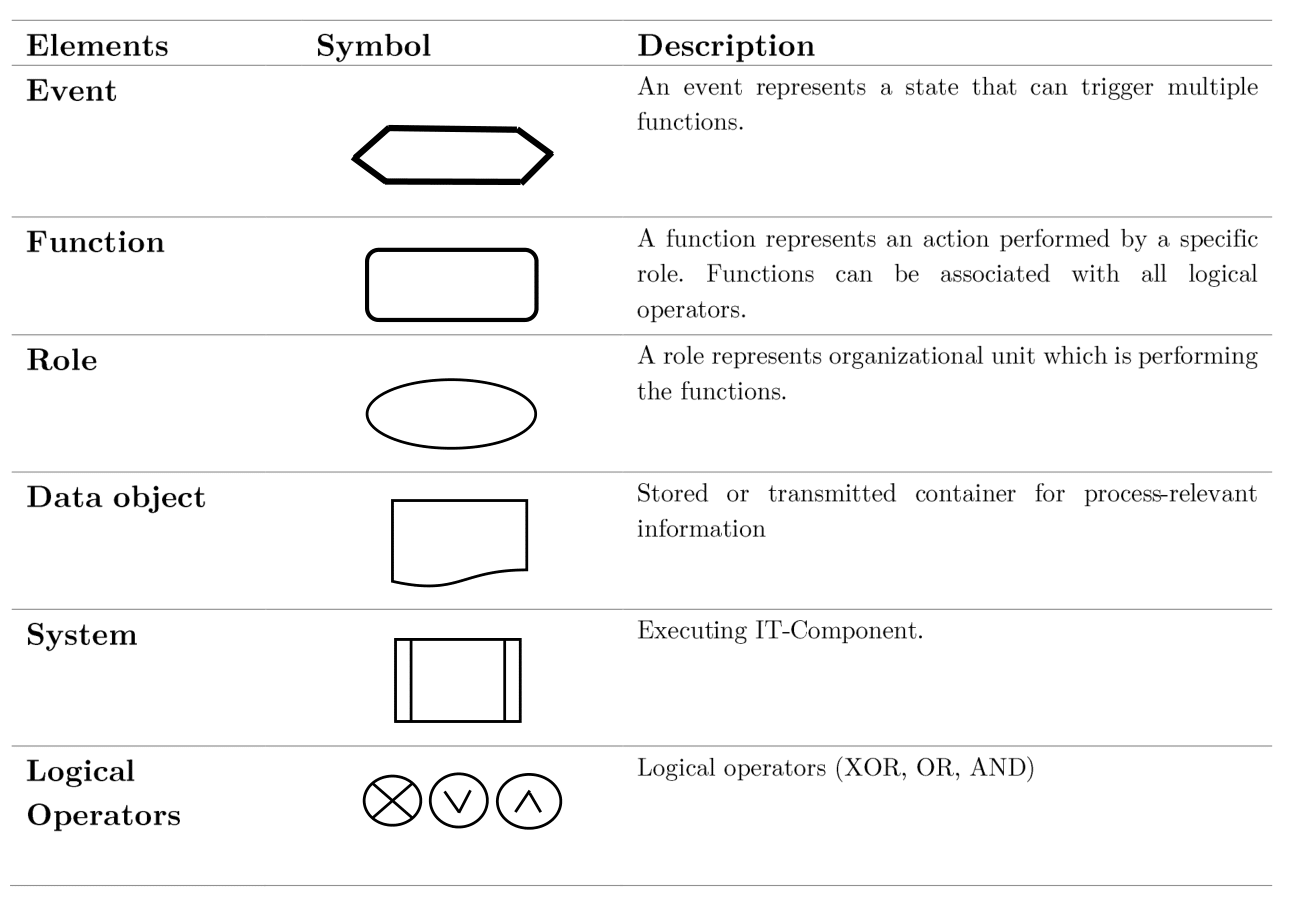
\includegraphics[scale=0.25]{EPC-1}
	\caption{Tabular arrangement of EPC model elements.}
\end{table}

Figure 2.4 shows the example model "buying bus ticket" with the EPC. The model clarifies which action is made by the user perfoming with the system and which action is made by the system itself. The first function is triggered by the user's desire to travel. The following steps depend on whether the user finds a destination or not. When he has located a destination for his trip, the system will show a number of ticket and payment options. The last action, performed by the user, requires the entry of money or credit card, so that the system can finally print the ticket.

\begin{figure}[!hb]
	\centering
	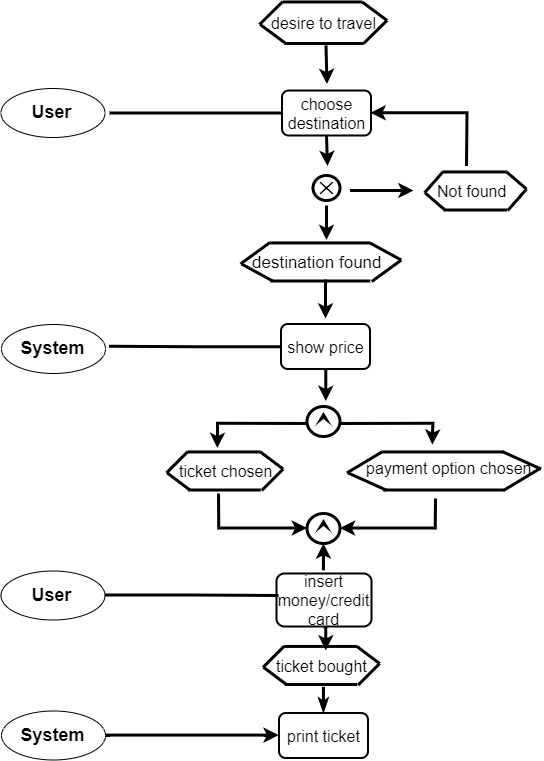
\includegraphics[scale=0.38]{EPC}
	\caption{Example of EPC with buying a ticket scenario.}
\end{figure}

% Das ist die Verknüpfung ins Abkürzungsverzeichnis


\newpage
\subsection{Business Process Model and Notation}
Before we approach the key point of this chapter, it is important to first understand the basic term of Business Process Management in more detail according to 'BPM Common Body of Knowledge'  \cite{EUROPEANASSOCIATIONOFBPM.2009}:

\par
\begingroup
\leftskip=1cm % Parameter anpassen
\noindent % Ab hier einzurückender Text
"Business Process Management is a systematic approach for capturing, designing, executing, documenting, measuring, monitoring and controlling both automated and non-automated processes in order to sustainably achieve the goals aligned with the corporate strategy.
BPM comprises the conscious and increasingly IT-supported determination,
Improvement, innovation and maintenance of end-to-end processes."
\par
\endgroup
Engineers often critisize the Business Process Model and Notation (\gls{Ccc}) that it cannot be related to structures such as IT landscape, data and strategies but therefore other forms of notations exist. While this is the case, BPMN should be applied towards process design and chronological sequence of activities. According to the book \cite{FREUND.2016}, the value chain is defined by processes that are represented by a collection of basic elements (Table 2.3).

\begin{table}[!hb]
	\centering
	\label{tbl:TableLatexShortened}
	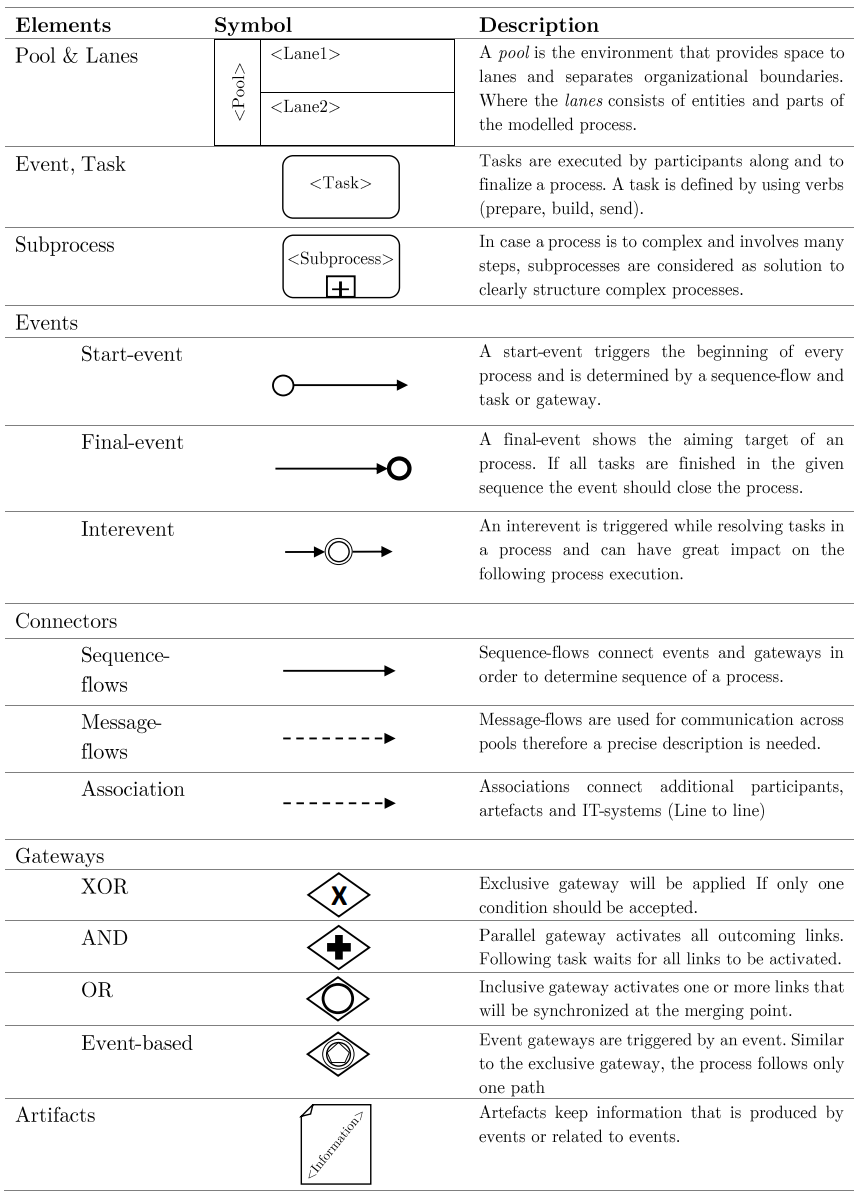
\includegraphics[scale=0.83]{TableBPMNLatex}
	\caption{Tabular arrangement of BPMN elements.}
\end{table}

\newpage
Numerous documentation \cite{DirkStahler.} and \cite{GeroDecker.} indicates that BPMN leads back to 2004 where the Business Process Management Initiative formalised this notation as a young standard to standardise interfaces of BPMS. The specification of BPMN is mainly focused on semi-formal characters and described in ISO/IEC 19510:2013. If we start to look from a global perspective towards BPMN, it is broadly acknowledged in the Anglo American areas that leads to preasure on EPC as a German formalised standard. Especially advantages like extensibality, seperation of control-/information flow in different lanes and a more formalised specification are advantages of BPMN.\\


\begin{figure}[!hb]
	\centering
	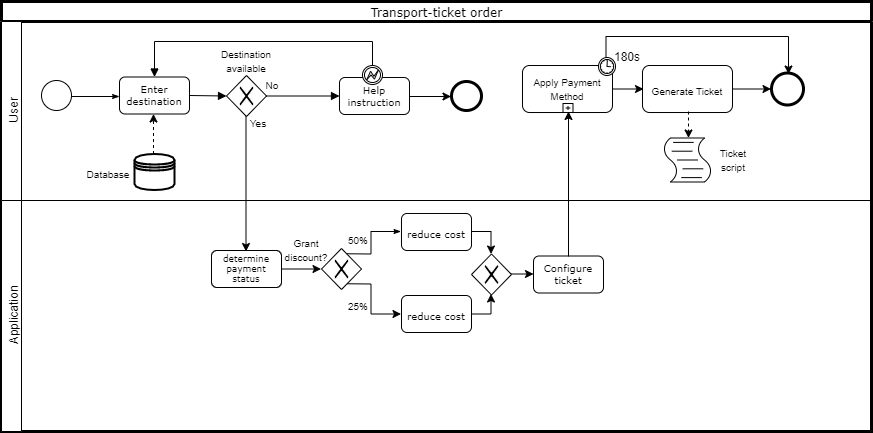
\includegraphics[scale=0.55]{BPMN_Ticket_Order}
	\caption{A ticket order process realised in a two lane pool by BPMN.}
\end{figure}

Above we look at a model for rising a transport ticket on a mobile application (Figure 2.5). As demonstrated by table 2.4, BPMN seperates the user environment from the machine environment in different lanes to support a clear understanding of roles and organizational entities that are included within the process. \\
Based on the prerequisite that a user is logged into the system before the actual process has been started the user lane is in control of avtivities like input, storage and a integrated subprocess payment method. First, the user input will be validated where the input is handled by an exclusive gateway and can be either true or false.\\
Now the process is handled by the application to consider special services and create an artefact.\
In the final step the task 'Apply payment method' is realised as a subprocess and is followed by the task 'Save ticket'.


%[Eur09] EUROPEAN ASSOCIATION OF BPM: Common Body of Knowledge for BPM. Schmidt (Götz), Wettenberg, 2009.



\newpage
\section{Behavioral perspective}
The final section considers modelling approaches with a behavioural perspective towards the system and describes embedments of a system in its system context. The outcome is a model that leads to understand the behaviour after events, condition changes or even effects coming from the system context towards the system.\cite{Pohl.2015}

\subsection{Petri net}
The basic model of the Petri net was introduced in the dissertation of Carl Adam Petri in 1962 \cite{Petri.1962} and was subsequently standardised in \cite{ISOIEC159091.122004}.
With its properties as a directed graph and disjunctive nodes (places and transitions) Petri nets allow graphical modelling and process simulation.\\
As a formal model for process modelling, the Petri net also has generic patterns following a semantic (table 2.5) in addition to the nodes. In the context of behavioural perspective state diagrams often appear as well. State diagrams use edges for transition modelling, while transitions in Petri nets belong to nodes. \cite{Winter.2013}\\

\begin{table}[!hb]
	\centering
	\label{tbl:TableLatexShortened}
	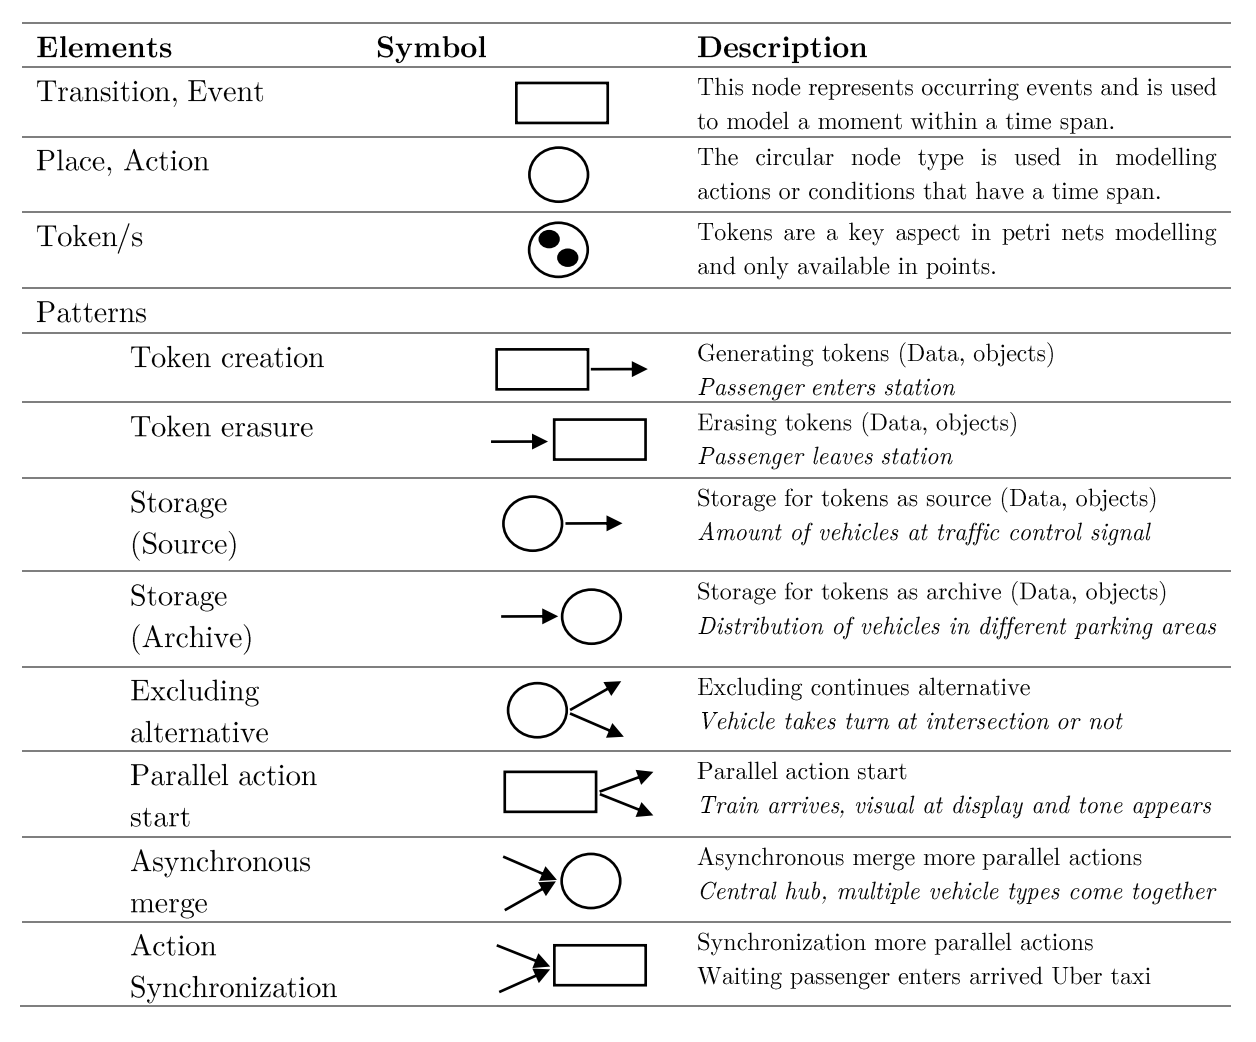
\includegraphics[scale=0.8]{petriTable}
	\caption{Tabular arrangement of Petri net elements.}
\end{table}

Tokens describe the capacity in the places and can be used for workflow modelling (time span). The capacity description shows the amount of storable tokens that can move over edges between the nodes, but is not permitted to violate the specified edge weight. \\
The transition is used for switching regulation and mapping events (moment in time span). One of the requirements for operations (AND, XOR) of a circuit is that previous digits fulfil the minimum quantity of edge weights and that there is sufficient residual capacity in the next place. Based on the edge weight, the circuit removes the required quantity of tokens from the previous place. \cite{Bernroider.2006}


\begin{figure}[!hb]
	\centering
	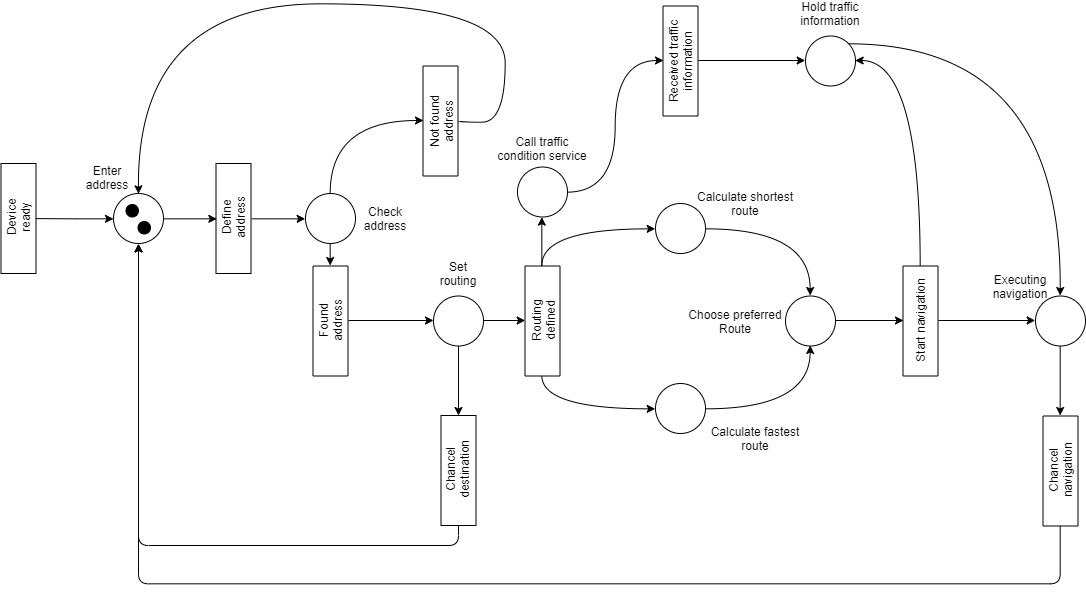
\includegraphics[scale=0.35]{PETRI-NET}
	\caption{A navigation system realised as a Petri net.}
\end{figure}

An illustration of a possible Petri net is shown in figure 2.6. It takes the use case of starting a route in a navigation system on a vehicle. This model can be seen as an active Petri net due its condition 'Enter address' keeps two tokens. Beyond that it is triggered by having an event 'Device ready'. \\
Passing the address check place for availability, a token either moves back to 'Enter address' or starts an activity 'Found address'. The model continous as excluding alternative in 'Chancel Destination' or 'Routing defined'. If not chanceled, multiple parallel activities will start 'Call traffic condition service' and route calculations, whereas route calculation is despite into two main route options before starting the navigation. While routing, the second token initialises traffic data service and holds this data in another action place. By the time the navigation starts the execution is provdided by traffic data. In case of a chanceled navigation the system prompts to enter a new address.


\newpage
\subsection{State diagram (UML)}
Based on the notation of Statecharts developed by \cite{DavidHarel.1987}, the \gls{Ggg} specified the model elements of the UML Statediagram in 2007. Both Statecharts and UML Statediagrams describe a technique to model the behavior of a system based on the concept of finite state machines. By definition, a finite state machine comprise a set of states and state transitions which, depending on the current state of the state machine, are executed by the occurrence of an event. A state defines a period of time in which the system under consideration shows a certain behavior and waits for the occurrence of a defined event. The change from one state to the next is triggered by events and is called state transition. Depending on the intended use, hierarchization in state machines allows to form superstates and to abstract from the possibly complex behavior in these states. [PR15] \\

\begin{table}[!hb]
	\centering
	\label{tbl:TableLatexShortened}
	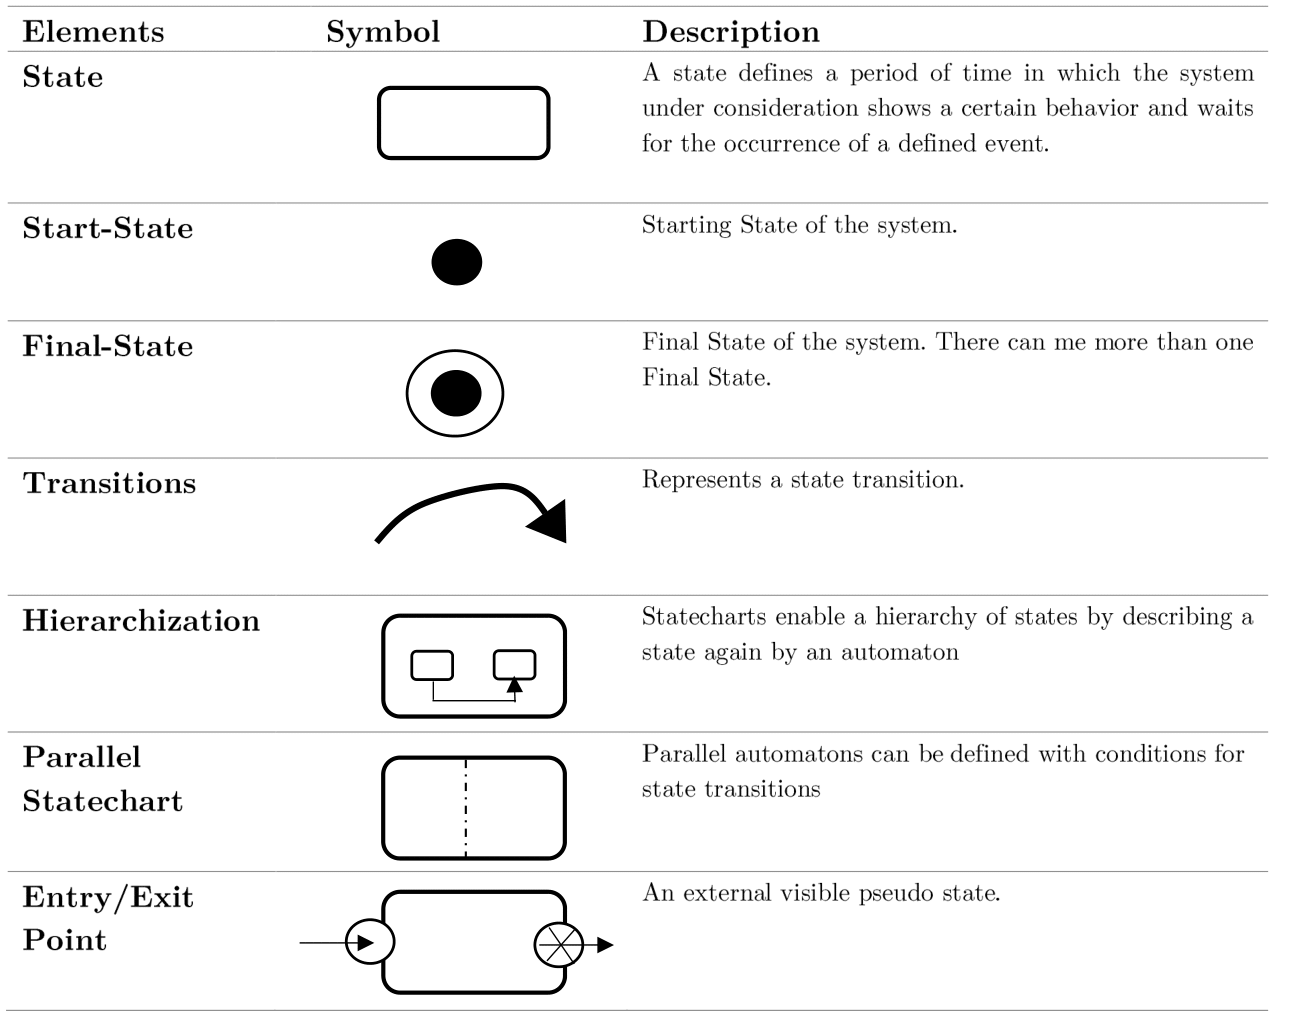
\includegraphics[scale=0.3]{statechart-1}
	\caption{Tabular arrangement of UML Statediagram elements.}
\end{table}

The UML 2 extends the model elements of statecharts by the possibility to define explicit entry and exit points for hierarchical states. \cite{Rumbaugh.1999} describe an entry point as an externally visible pseudo state that is directly associated with an internal state. An exit point as an externally visible pseudo state that has an internal state as its origin. A superstate within a state machine can have any number of entry and exit points defined by a name.

\newpage
Figure 2.7 shows a modelled scenario of a navigation device. The initial state is when the navigation device is ready. The next State Transition is triggered by the users decision whether he wants to be navigated to a new destination or the last destination set in the system. Both decision end in the superstate "Route calculation". There is a loop between "Route calculation" and "Display Route", because the Route has to be permenatly updated. The final state and at the same time the initial state is reached when navigation is aborted or successfully completed.\\

\begin{figure}[!hb]
	\centering
	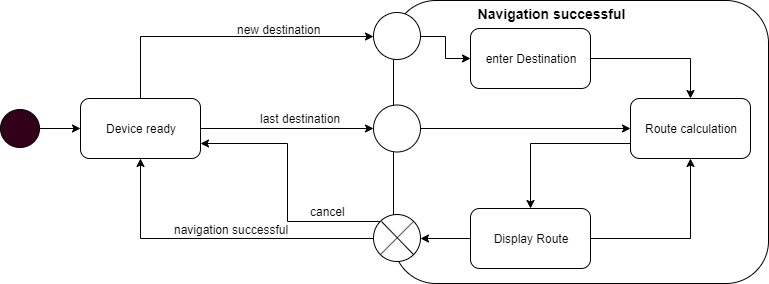
\includegraphics[scale=0.55]{UMLState}
	\caption{State diagram with navigation device scenario.}
\end{figure}

\chapter{Workflow engines}

\section{jBPM}
Java Business Process Management is a free open source workflow management framework developed by JBoss, based on Java language. jBPM is an lightweight, open source, flexible, easily extensible executable process language framework that covers business process management, workflow, and service collaboration. jBPM mainly includes Workflow Engine, flow monitoring tool and Graph Process Designer based on Eclipse platform. \cite{.2018}.
 \cite{ParedesVillegas.1993}
 
\begin{enumerate} %[!hb]
	\item \textbf{Workflow Enginge} 
	\\The workflow engine controls the runtime process, provides interfaces for process definition, process management and process monitoring and user interfaces through which systems can interact with the workflow engine. As shown in Figure 3.1
	It is designed with a layered architecture.
	The engine consists of the four core classes Execution Service, Task Service, History Service and Identity Service \cite{.2018}
	\item \textbf{Process Designer}
	\\This is an Eclipse plug-in, which provides support for defining
	processes in jPDL both in a graphical format and in XML. \glspl{jpdl} is the process language used by the system. \cite{TerHofstede.2010}
	\item \textbf{Workflow Client}
	\\ It is a
	web-based client through which users can initiate processes and execute activities through an API.
	The user interface also allows administrators to monitor processes and instances. Furthermore, the Identity component, takes care of	the definition of organizational information, such as users, groups, and roles.\cite{TerHofstede.2010}

\end{enumerate}


\newpage
jBPM enables flexibility by supporting
multiple-process languages with the same scalable process
engine platform. jBPM not only supports jPDL but also other 
XML-based process languages like: \gls{WSBPEL} and Seam Pageflow. \cite{Zhang.2008}
\\

\begin{figure}[!hb]
	\centering
	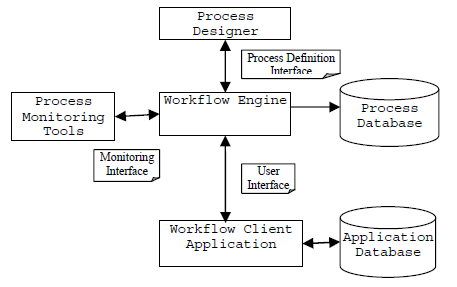
\includegraphics[scale=0.85]{jBPM}
	\caption{Overview jBPM components. \cite{ParedesVillegas.1993}}
\end{figure}

According to \cite{.2018} a basic flow of jBPM workflow enginge consists of the components shown in Figure 3.2. First
define the process that meets the needed business requirements. When the
process is defined, use the graphical
process designer to draw the business process. It is possible to use the designer
to generate the jPDL or directly write the XML document
corresponding to the jPDL. The jBPM workflow engine creates
process instances depending on the underlying jPDL or XML. Then,
according to a specific business, a business document report
can be created. Users can invoke the relevant interfaces
provided by jBPM to realize the specific process operations of
the enterprise through the system interface.

\begin{figure}[!hb]
	\centering
	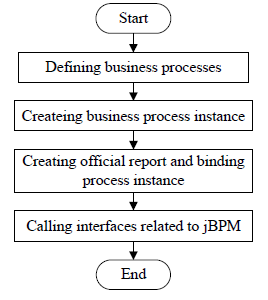
\includegraphics[scale=0.85]{jBPMworkflow}
	\caption{basic flow of the JBPM workflow enginge. \cite{.2018}}
\end{figure}
\newpage
Using the fundamental engine and modal behind jBPM, Red Hat developed a Process Automation Manager which comes with a higher performance. The Process Automation Manager is a platform for developing containerized microservices and applications that automate business decisions and processes. \cite{RedHat.2019} The Laser Group, in partnership with Red Hat, introduced the Process Automation Manager to streamline business processes.
Figure 3.3 shows the transformed business process by using the Process Automation Manager.
The \gls{IVR} now sends all information to the Process Engine, which addresses the respective responsible service. \\

\begin{figure}[!hb]
	\centering
	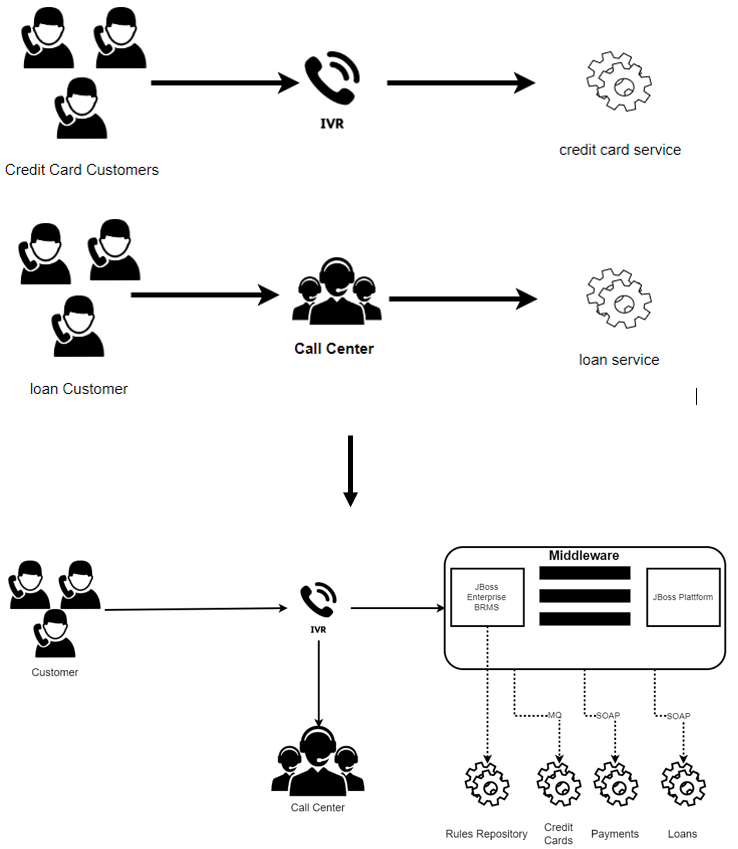
\includegraphics[scale=0.6]{RedHatnew}
	\caption{Business transformation by using Process Automation Manager.}
\end{figure}


\newpage
\section{Camunda}
The Camunda stack provides a toolset of execution and decision engines for BPM workflows and process modelling so that projects can be structured, automated and executed. Enterprises and institutions of various industries like corporate, startups and public with medium to large size, a complex IT landscape and strives for automated processes benefit from Camundas components. \cite{RobertGimbel.20.2.2019} \\
The Java-based framework orchestrates and supports agile and common open source services to enable a better work environment for various team roles: System architects, software engineers, project manager and business analysts. Figure 3.3 illustrates the Camunda infrastructure and components together with typical team roles (developer, manager, analyst), implemented standards (BPMN, DMN) and architectural functionalities (container-managed Java engine). \cite{CamundaServicesGmbH.2019}

\begin{figure}[!hb]
	\centering
	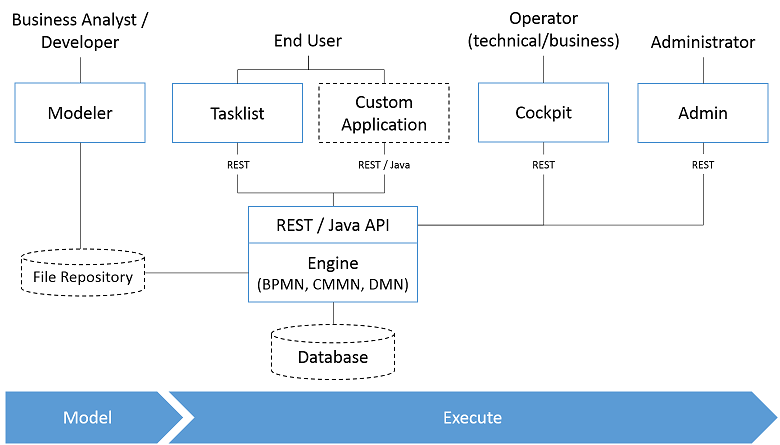
\includegraphics[scale=0.65]{CamundaArchitecture}
	\caption{Overview Camunda components. \cite{CamundaServicesGmbH.2019}}
\end{figure}

Camunda Modeler is a high-level modelling tool based on \gls{Hhh}, \gls{Iii} and \gls{Jjj} standards that embraces analysts and developers to design processes given by projects or enterprise strategies. An integrated \gls{Mmm} and \gls{Lll} service enables a local repository to bridge deployments between the Camunda Modeler (\gls{Nnn} formatted process) and the executing engine. Camunda has a lightweighted engine that is responsible to execute given tasks and decisions. In addition, Camunda provides an open source REST interface for requesting web applications. Provided or self-customized web applications provide components that manage workflow tasks (Tasklist), process monitoring and error handling (Cockpit) and authorization (Admin) functionalities. \cite{CamundaServicesGmbH.2019} 

\newpage
Best practices of Camunda can be found in IT solutions with any project context in order to initiate, plan, control and evaluate individual process automation or detect system related gaps.
This section focuses on the Camunda integration towards stages of a technology-driven project. \cite{RobertGimbel.20.2.2019} 

\begin{enumerate} %[!hb]
\item \textbf{Project Scoping} 
\\Views on project scoping range from project objectives to practical activities to define costs of errors and manual work, quality of transparency, throughput, time to market and adaptions. 
Camunda is used to give a pre-study about project volume and risks which is a certain need in the stage of proofing a concept. Equally important is communication between team roles that negotiate project vision by BPMN and DMN.
\item \textbf{Design and Implementation}
\\Next stage is design and implementation to accumulate functional and non-functional requirements in an incrementally approach. Besides that, the team roles and tasks are defined and introduced to domain knowledge. Camunda will be technically integrated into consisting architecture. Whereas existing instances of processes, decisions and optimisations are modelled and maintained against performance issues. 
\item \textbf{Solution Rollout}
\\A solution rollout expects a closed test cycle and acceptance by management before released to operations. Now, release and change management take over and ensure security, version control and monitoring enabled by Camunda Cockpit.
\item \textbf{Continuous Improvement}
\\As result the automated process can be continuously improved by analysing operational data, \gls{Ooo} monitoring and error handling. Camundas retrospectively function helps to identify enhancements, weak points and capacity planning of affected components.
\end{enumerate}

Looking at the case study of Deutsche Telekom \cite{FriedbertSamland.}, a German telecommunications company, Camunda has been partially applied to break down a system from monolytical architecture into a microservice based architecture. Historically, the issue focussed on a inflexible IT landscape of a TAL-order process back in 2008 that shall be reengineered for fiber-optic communication by a new service oriented architecture. In 2018, leading engineers identified 4 main drivers to this project: \textit{\gls{Qqq}}, \textit{\gls{SAFe}} to enable bottom up and top down workflow, \textit{Cloud} technology reduces maintanance, provides scalability and self service and \textit{\gls{DEVOP}} to manage complex application stacks.

\newpage
Following the microservice architecture (MSA) vision, the existing monolith partitions into self-suistaining and lightweighted services. This was achieved by categorise into frontend-/ business-/ backend data, group functionalities to ensure consistent order processing, data calculations and finally, define and assign three microservice categories: Business process microservice (incl. Camunda), data microservice and domain microservice (incl. Camunda). \\[1em]
The meshed solution is provided by two independent coordination patterns of services. Unfortunately, a orchestrated solution was not suitable due its centralised BPM engine. Furthermore, a choreography oriented solution has had advantages in its loose coupling but disadvantages in locating processes and orders. To conclude, the final solution is a 'choreographed orchestration' which enables each microservice component to keep a BPM engine while communicating with a messaging broker.
[\cite{CamundaServicesGmbH.May2017}, \cite{FriedbertSamland.}]\\
These factors contribute to a more performant architecture with lightweighted and Java-based development, supports exception handling in operations and influences IT-Business alignment by visualizing complex logic. \\

\begin{figure}[!hb]
	\centering
	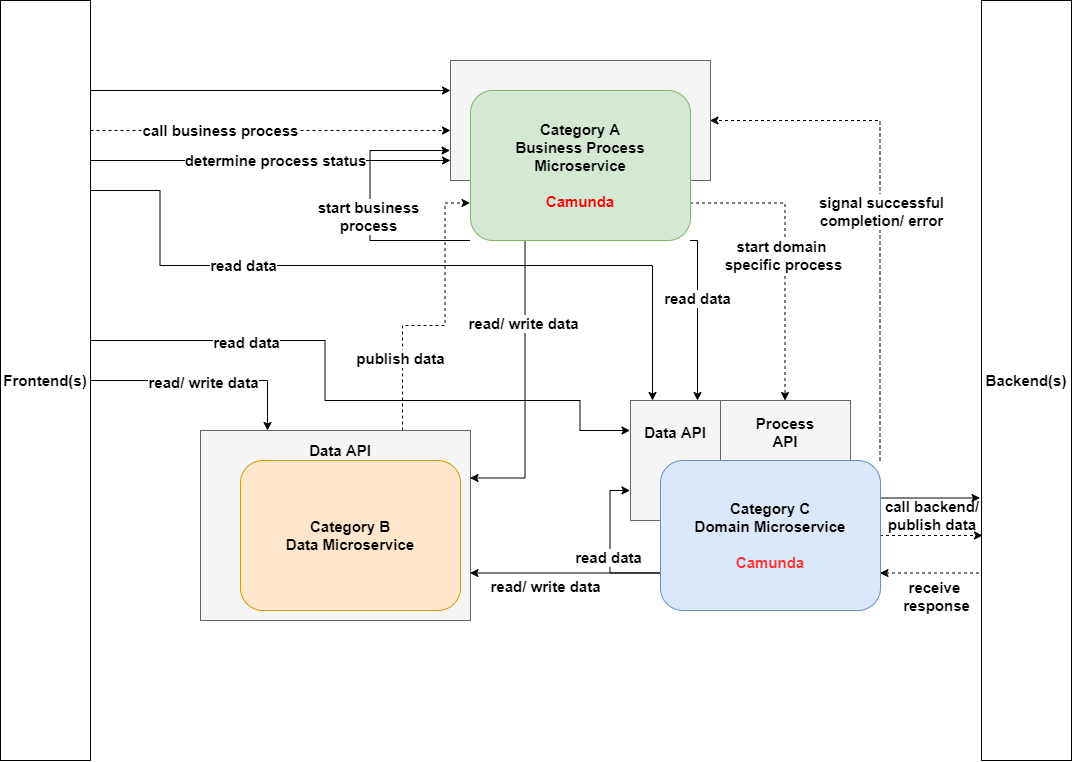
\includegraphics[scale=0.4]{CamundaBPMN}
	\caption{MSA of implemented solution with Camunda engines. \cite{FriedbertSamland.}}
\end{figure}


\chapter{Conclusion}

The different perspectives show that, depending on the use case, it is possible to choose from a pool of modelling languages. When it comes to the structural perspective, the use of UML class diagrams has proven to be a good choice. ER models are therefore no worse than UML class diagrams; they address a different domain. For example, they are consistent when it comes to lightweight modeling of relations.
In the modeling of the functional perspective, we can observe that BPMN is used more in companies for business process modeling, since BPMN allows the modeling of more complex processes due to the specification. Furthermore, it is because there are workflow engines for BPMN. The presented modelling languages of the behavioural perspective behave similar to those of the structural perspective. Modelling with Petri nets has been done since 1960. The corresponding UML was specified much later, which is significantly reflected in the understanding of the language. When it comes to modeling workflows, Petri nets address active systems, rather than reactive ones. Furthermore Petri nets can be described mathematically, which makes them interesting for mathematical models. 
\\
The following table 4.1 illustrates a functional comparative of the workflow engines Camunda and jBPM. Both provide a graphical modeler, but do not offer the possibility to add functionality. Depending on the system context, developers decide which engine is more suitable for the use case. 

\begin{table}[!hb]
	\centering
	\label{tbl:TableLatexShortened}
	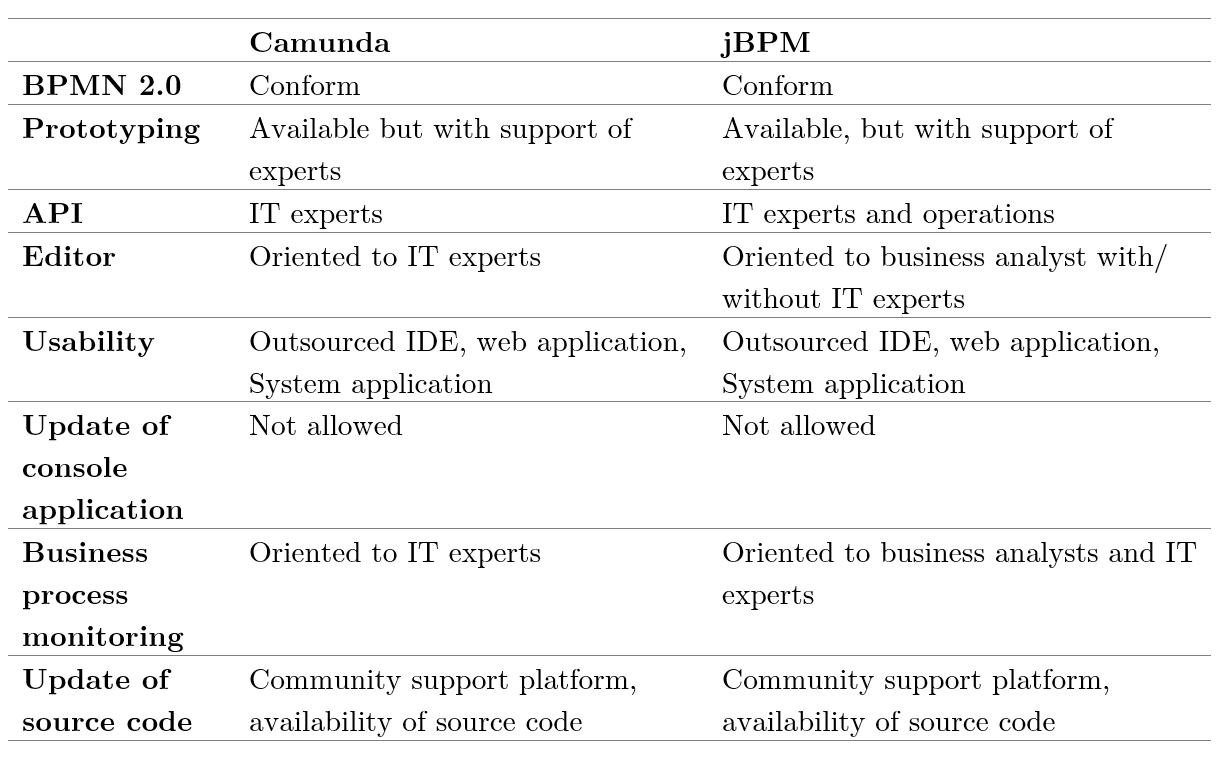
\includegraphics[scale=0.75]{EngineTable}
	\caption{Comparison of the workflow engines Camunda and jBPM.}
\end{table}



%\section{Prospect}
%<content>



 % Beispiel
\end{onehalfspacing}

%% Optional: Anhang
%\appendix
%\include{anhang_a}
%\include{anhang_b}

\cleardoublepage

%% Literatur
\addcontentsline{toc}{chapter}{\bibname}

\pagenumbering{Roman}
\setcounter{page}{7}
\IfLanguageName{ngerman}{
\bibliographystyle{em_includes/emalphde}
% Alphanumerische Zitierung (EM Style), deutsch. Ggf. durch andere Varianten 
% im Ordner em_includes austauschen.
}{
\bibliographystyle{em_includes/emalphen}
% Alphanumeric Citation (EM Style), English.
}

%\nocite{*} % Alle Quellen anzeigen, die im Bibfile stehen, auch wenn sie nicht im Text referenziert wurden
\bibliography{literature}

%% Index
%\addcontentsline{toc}{chapter}{\indexname}
%\printindex            % Index, Stichwortverzeichnis
%\end{onehalfspacing}
\end{document}
%% end of file
